For the first part of this chapter, we consider ""multidimension quantitative games"". With regard to the formalism of~\cref{chap:payoffs}, the only change to the arena is the set of colours associated with edges: we now have vectors in $\R^k$ where $k \in \N_{>0}$ is the ""dimension"" of the game. As before, for computational purposes, it makes sense to restrict our colouring to rational numbers, and for the sake of simplicity, we even consider \emph{integers only} without loss of generality.

For the weighted games of~\cref{chap:payoffs}, where a single quantitative objective $f$ is considered, we know that the "value" of the game exists. In most cases, optimal strategies do too, which makes the problems of computing the value and solving the game for a given threshold morally equivalent. In our simple multidimension setting, we focus on \emph{conjunctions} of objectives. Similarly to what we did in the one-dimension case, we will write $f_{\geq \vec{x}}$ with $\vec{x} \in \Q^k$ to define the objective
\[
f_{\geq \vec{x}} = \bigcap_{i = 1}^{k} \left\lbrace \play \in E^\omega \mid f_i(\play) \geq \vec{x}_i\right\rbrace 
\]
where $f_i(\play)$ represents the evaluation of $f$ on the sequence of colours in the $i$-th dimension and $\vec{x}_i$ represents the $i$-th component of vector $\vec{x}$. Hence we consider the natural semantics where we want to satisfy the original objective $f$ component-wise.

\begin{example}
\label{12-ex:MMP}
Consider the simple one-player game in~\cref{12-fig:MultiMP} fitted with the "mean-payoff" objective $\MeanPayoff^-$  (recall that two variants exist depending on the use of lim-sup or lim-inf). \todo{Notation issue should be solved in Benjamin/Petr's chapters. Add ref here.} Let us first recall that in the single-objective case, memoryless strategies suffice to play optimally (\cref{4-thm:mean_payoff_positional}). In this game, such strategies permit to achieve payoffs $(1,-1)$, $(-1,-1)$ and $(-1,1)$. Intuitively, $(-1,-1)$ is not interesting since we can do better with $(1,-1)$ or $(-1,1)$. On the other hand, these two other payoffs are incomparable and thus should not be discriminated a priori. In the multiobjective world, there is usually no total order between the outcomes of a game -- fixing a total order would actually boil down to transforming the game into a one-dimension game -- which is why there is in general no optimal strategy but rather \emph{Pareto-optimal} ones. Intuitively, a strategy is Pareto-optimal if there exists no other strategy yielding a payoff which is as good in all dimensions and strictly better in at least one dimension.
\end{example}

\begin{definition}[""Pareto-optimal strategy""]
Given a $k$-dimension game $\game$ based on the conjunction of $k$ maximising (w.l.o.g.) quantitative objectives $(f_i)_{i=1}^{k}$, a strategy $\sigma$ for Eve is said to be \emph{Pareto-optimal} if it guarantees a payoff $\vec{x} \in \R^k$ such that for all other strategy $\sigma'$ of Eve ensuring payoff $\vec{x}' \neq \vec{x}$, it holds that $\vec{x}_i > \vec{x}'_i$ for some dimension $i \in \{1, \ldots, k\}$.
\end{definition}
 
  
\begin{figure}[tbp]
  \centering
  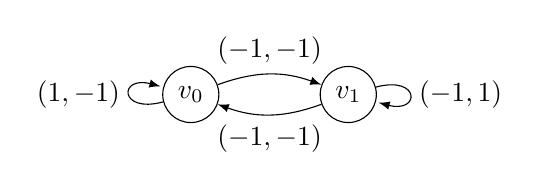
\begin{tikzpicture}[node distance=2cm,>=latex]
    \node[draw,circle](1) {$v_0$};%
    \node[draw,circle,right of=1](2) {$v_1$};%

    \path[->] (1) edge[bend left=20] node[above] {$(-1,-1)$} (2)%
    (2) edge[bend left=20] node[below] {$(-1,-1)$} (1)%
    (1) edge[loop left] node[left] {$(1,-1)$} (1)%
    (2) edge[loop right] node[right] {$(-1,1)$} (2);%

  \end{tikzpicture}
  \caption{A simple multidimension mean-payoff game where Eve needs infinite memory to play (Pareto-)optimally.}
  \label{12-fig:MultiMP}
\end{figure}

The concept of Pareto-optimality has an important consequence on multiobjective problems: the correspondence between solving a threshold problem and computing an optimal strategy that holds in the single-objective case does not carry over. Indeed, one may now be interested in computing the ""Pareto frontier"" consisting of all Pareto  vectors achievable by Eve. This comes at great cost complexity-wise as this frontier may include many points, and in some settings, even an \emph{infinite number of Pareto vectors} (see~\cref{12-sec:percentile} for an example), \todo{Add direct ref when done.} sometimes forcing us to resort to approximation. This requires specific techniques that go beyond the focus of this chapter, hence in the following we mostly discuss the \emph{"threshold problem"}, also referred to as ``solving the game'' for a given threshold vector.

\begin{example}
\label{12-ex:MMP2}
Let us go back to~\cref{12-ex:MMP} and fix objective $\MeanPayoff^{-}_{\geq \vec{x}}$ where $\vec{x} = (0, 0)$. As discussed before, this threshold cannot be achieved by a memoryless strategy. Actually, this is also the case for any \emph{finite-memory} strategy. Indeed, any finite-memory strategy induces an ultimately periodic play, where either (a) the periodic part only visits $v_0$ (resp.~$v_1$), yielding payoff $(1,-1)$ (resp.~$(-1,1)$) thanks to "prefix independence" (\cref{chap:payoffs}), or (b) it visits both in which case the mean-payoff is of the form
\[
\vec{y} = \MeanPayoff^{-}(\play) = \dfrac{a \cdot (1, -1) + 2 \cdot b \cdot (-1, -1) + c \cdot (-1, 1)}{a + 2 \cdot b + c}
\]
where $a, c \in \N$ and $b \in \N_{>0}$. Observe that $\vec{y}_1 + \vec{y}_2 = -4\cdot b / (a + 2 \cdot b + c)$, which is strictly less than zero for any value of the parameters. Hence $\vec{x} = (0, 0)$ is not achievable. Now consider what happens with infinite memory: let $\sigma$ be the strategy of Eve that visits $\ell$ times $v_0$, then $\ell$ times  $v_1$, and then repeats forever with increasing values of $\ell$. The mean-payoff of the resulting play is the limit of the previous equation when $a = c = \ell$ tends to infinity, with $b = 1$: intuitively, the switch between $v_0$ and $v_1$ becomes negligible and the mean-payoff is $\frac{1}{2} \cdot (1,-1) + \frac{1}{2}\cdot(-1,1) = (0, 0)$.
\end{example}

\begin{remark}
While Eve cannot achieve $(0, 0)$ with finite memory, she can achieve (i.e., ensure at least) any payoff $(-\varepsilon, -\varepsilon)$ for $\varepsilon > 0$, using sufficient memory: for instance, by taking $b = 1$ and $a = c = \lceil \frac{1}{\varepsilon} - 1\rceil$ (if $\varepsilon \geq 1$, any strategy works so $a = b = 0$ is fine). In that sense, the payoff $\vec{x} = (0, 0)$ achievable by an infinite-memory strategy can be seen as the supremum of payoffs achievable by finite-memory strategies. Actually, this is exactly how we defined strategy $\sigma$: Eve plays according to an infinite sequence of finite-memory strategies parametrised by $\ell$, such that each strategy of the sequence ensures mean-payoff $(-\varepsilon, -\varepsilon)$, with $\varepsilon \to 0$ when $\ell \to \infty$.
\end{remark}

\begin{example}
\label{12-ex:MMP3}
The reasoning above holds similarly for $\MeanPayoff^{+}$. With finite-memory, the lim-sup variant coincides with the lim-inf one: because the play is \textit{ultimately periodic}, the limit exists. With infinite-memory, Eve can actually achieve the payoff $\vec{x}' = (1, 1)$, witnessing a gap with the lim-inf variant. To do so, she has to play a strategy that alternates between $v_0$ and $v_1$ while staying in each vertex for a sufficiently long period such that the current mean over the corresponding dimension gets close to $1$. Getting these means closer and closer to $1$ and using the lim-sup component-wise then suffices to achieve payoff $\vec{x}'$. For instance, starting in~$v_0$, Eve could choose  $v_1$ 10 times to reach mean $0.9$ on the second dimension, then choose $v_0$ 2189 times to reach mean $0.99$ on the first dimension, and so on. This is in stark contrast to the lim-inf variant, which cannot achieve any payoff $(\varepsilon, \varepsilon)$ for $\varepsilon > 0$ (the Pareto vectors correspond to linear combinations of simple cycles, as hinted before).
\end{example}

\begin{theorem}
\label{12-thm:MMP-Eve}
Multidimension mean-payoff games require infinite-memory strategies for Eve. Furthermore, the lim-inf and lim-sup variants are not equivalent, i.e., their winning regions are in general not identical.
\end{theorem}

This theorem already shows the first signs of our single-objective assumptions crumbling in the multiobjective world: we jump from memoryless determinacy to needing infinite memory, and objectives that were equivalent both in games and MDPs turn out to be different here. Buckle up, as this was only our first step.
